% Copyright 2005-2016 Airbus-EDF-IMACS-Phimeca
% Permission is granted to copy, distribute and/or modify this document
% under the terms of the GNU Free Documentation License, Version 1.2
% or any later version published by the Free Software Foundation;
% with no Invariant Sections, no Front-Cover Texts, and no Back-Cover
% Texts.  A copy of the license is included in the section entitled "GNU
% Free Documentation License".
\renewcommand{\filename}{docUC_StocProc_StationaryCovarianceFunction_UserDefined.tex}
\renewcommand{\filetitle}{UC : Creation of a  User defined stationary covariance function}

% \HeaderNNIILevel
% \HeaderIILevel
\HeaderIIILevel

\label{StationaryCovarianceModelCreation}
\index{Stochastic Process!Covariance Model}

This use case illustrates how the User can define his own stationary covariance model.\\

A stationary covariance model $C^{stat}$ is defined by : $C^{stat}:  \cD \rightarrow  \mathcal{M}_{d \times d}(\Rset)$ where  $C^{stat}(\vect{\tau})$ is a covariance matrix of dimension $d$. \\
Note that $\cD=\Rset^n$ in the continuous case and $\cD$ is a lattice in the discrete case.\\


OpenTURNS allows the User to define his own stationary covariance model thanks to the object {\itshape UserDefinedStationaryCovarianceModel} defined from :
\begin{itemize}
\item a mesh $\cM$ of dimension $n$ defined by the vertices $(\vect{\tau}_0,\dots, \vect{\tau}_{N-1})$ and the associated simplices,
\item a collection of covariance matrices stored in the object \emph{CovarianceMatrixCollection} noted $(\mat{C}_0, \dots, \mat{C}_{N-1})$ where $\mat{C}_k \in \mathcal{M}_{d \times d}(\Rset)$ for $0 \leq k \leq N-1$.
\end{itemize}
Then OpenTURNS builds a stationary covariance function which is a piecewise constant function on $\cD$ defined by:
\begin{align*}
  \forall \vect{\tau} \in \cD, \, C^{stat}(\vect{\tau}) =  \mat{C}_k \mbox{ where } k \mbox{ is such that } \vect{\tau}_k \mbox{ is the  vertex of } \cM  \mbox{ the nearest to } \vect{t}.
\end{align*}


Care: in its version 1.3, OpenTURNS only implements the case $n=1$ where the mesh
$\cM$ is a regular time grid $(t_0, \dots, t_{N-1})$ discretizing $\cD=[0,T]$.\\




\requirements{

  \begin{description}
  \item[$\bullet$] a mesh : {\itshape myShiftMesh}
  \item[type:]  Mesh
  \end{description}

  \begin{description}
  \item[$\bullet$] a collection of covariance matrices : {\itshape myCovarianceCollection}
  \item[type:]  CovarianceMatrixCollection
  \end{description}

  \begin{description}
  \item[$\bullet$] one vertex : {\itshape tau}
  \item[type:]  NumericalPoint
  \end{description}

}
{
  \begin{description}
  \item[$\bullet$] a stationary covariance model : {\itshape myCovarianceModel}
  \item[type:] StationaryCovarianceModel
  \end{description}

}

\textspace\\
Python script for this UseCase :

\inputscript{script_docUC_StocProc_StationaryCovarianceFunction_UserDefined}

\textspace\\




In the following example, we illustrate how to create a covariance model of dimension $d=1$ and when the domain $\cD=[0,T]$.\\
We model the covariance function defined by: $C^{stat}:\Rset \rightarrow  \Rset$ where $C^{stat}(\tau) = \frac{1}{1 + \tau^2} $. In this example, the domain $\cD$ is with $[0,20]$ discretized with the time step $\Delta t = 0.5$.\\


The Figure \ref{UserDefinedStationaryCovarianceModelDemonstration} draws the covariance function.

\begin{figure}[H]
  \begin{center}
    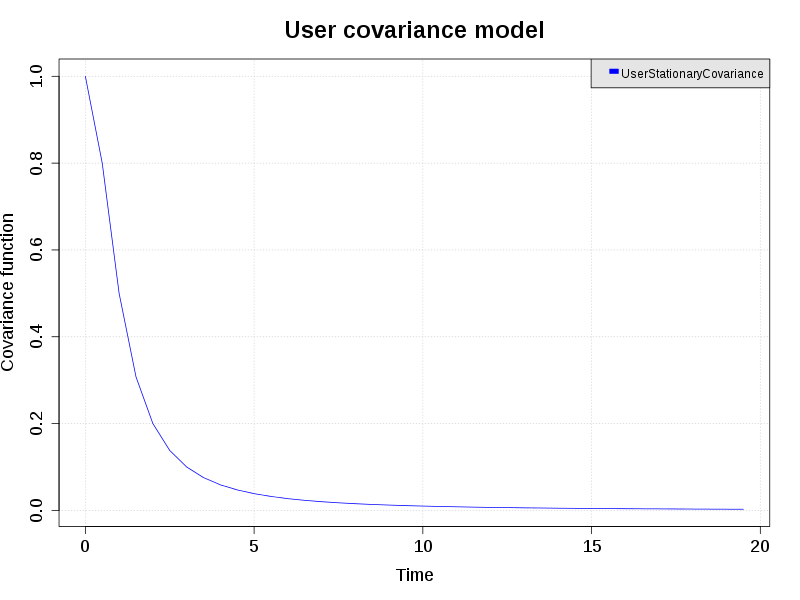
\includegraphics[width=7cm]{Figures/UserDefinedStationaryCovarianceModelDemonstration.png}
    \caption{User defined stationary covariance model in dimension 1 when $\cD=[0,T]$.}
    \label{UserDefinedStationaryCovarianceModelDemonstration}
  \end{center}
\end{figure}
